%!TEX root = ../thesis.tex

\section{ハードウェア}
本研究では, 屋外自律高速モビリティを制御対象とする.
モビリティは差動二輪と従動輪で構成された三輪モデルであり, 駆動モータの動作に追従するような従動輪機構となっている.
Fig.3.1に外装を取り付けたモビリティと外装を取り外したモビリティのハードウェアの外観を示す.

\begin{figure}[h]
     \centering
     \begin{minipage}[c]{65mm}
         \centering
         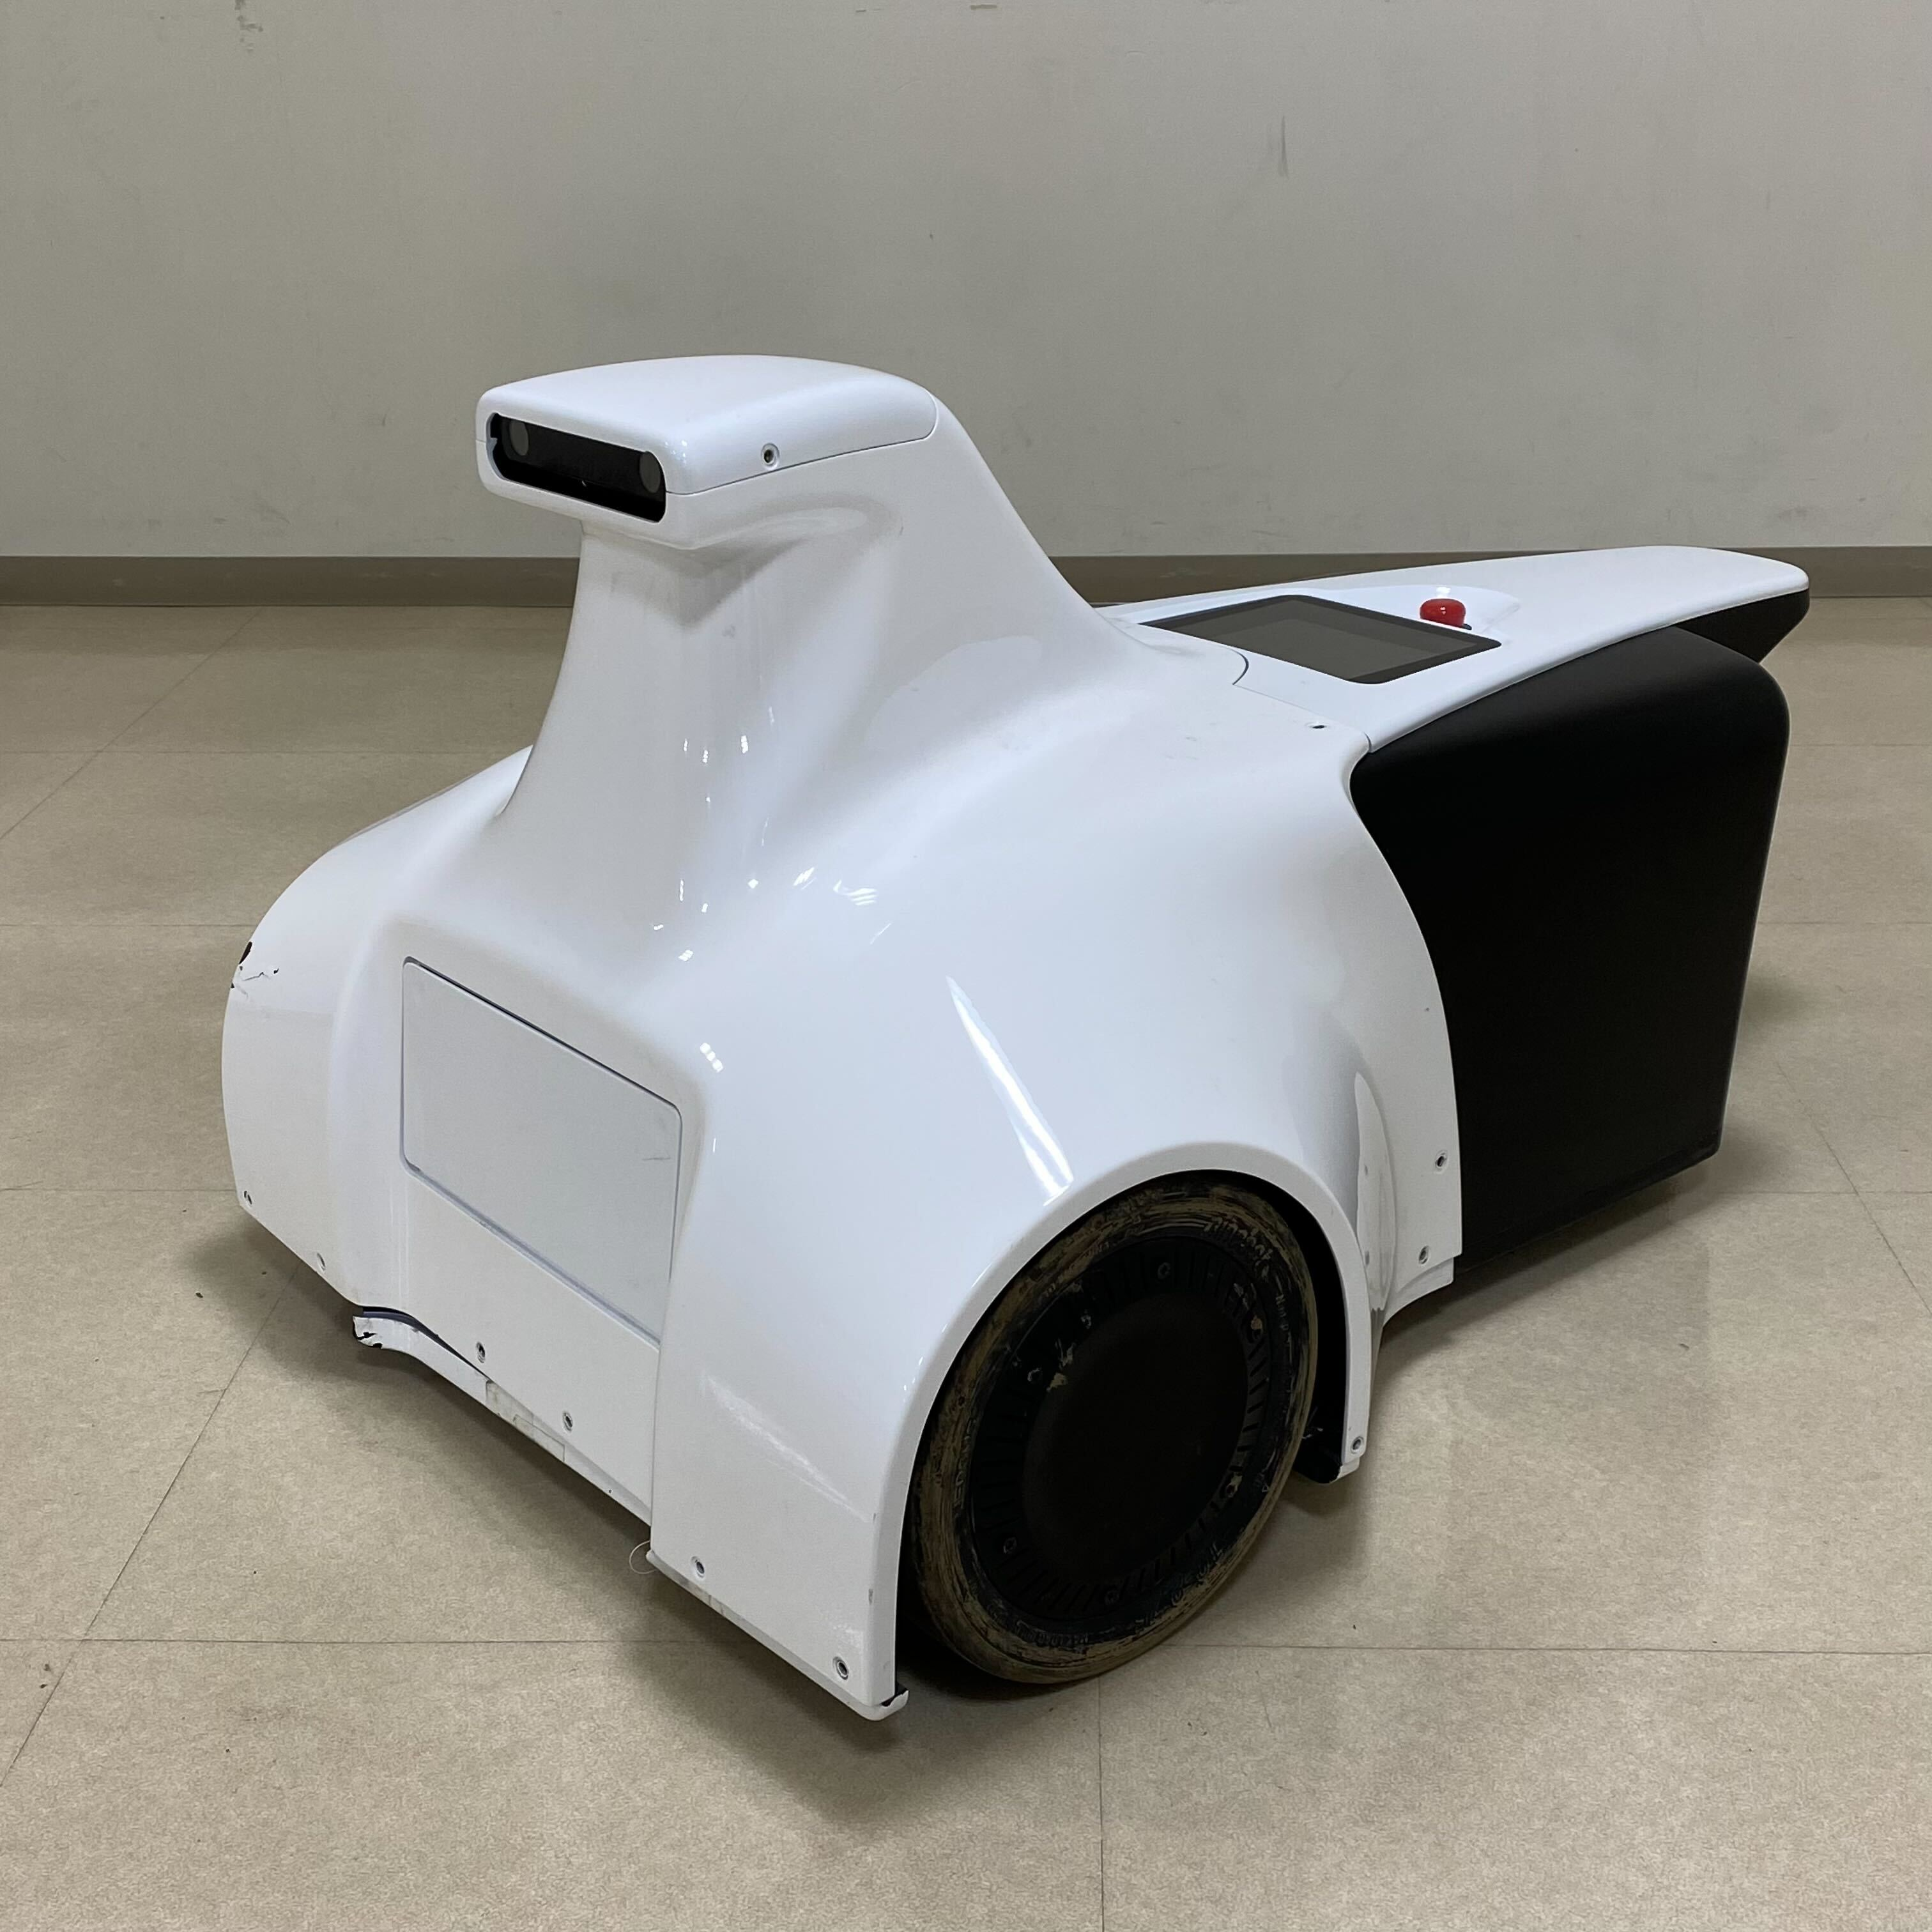
\includegraphics[height=50mm]{images/robotwithexterior.png}
         \subcaption{Mobility with exterior}
     \end{minipage}
     \begin{minipage}[c]{65mm}
         \centering
         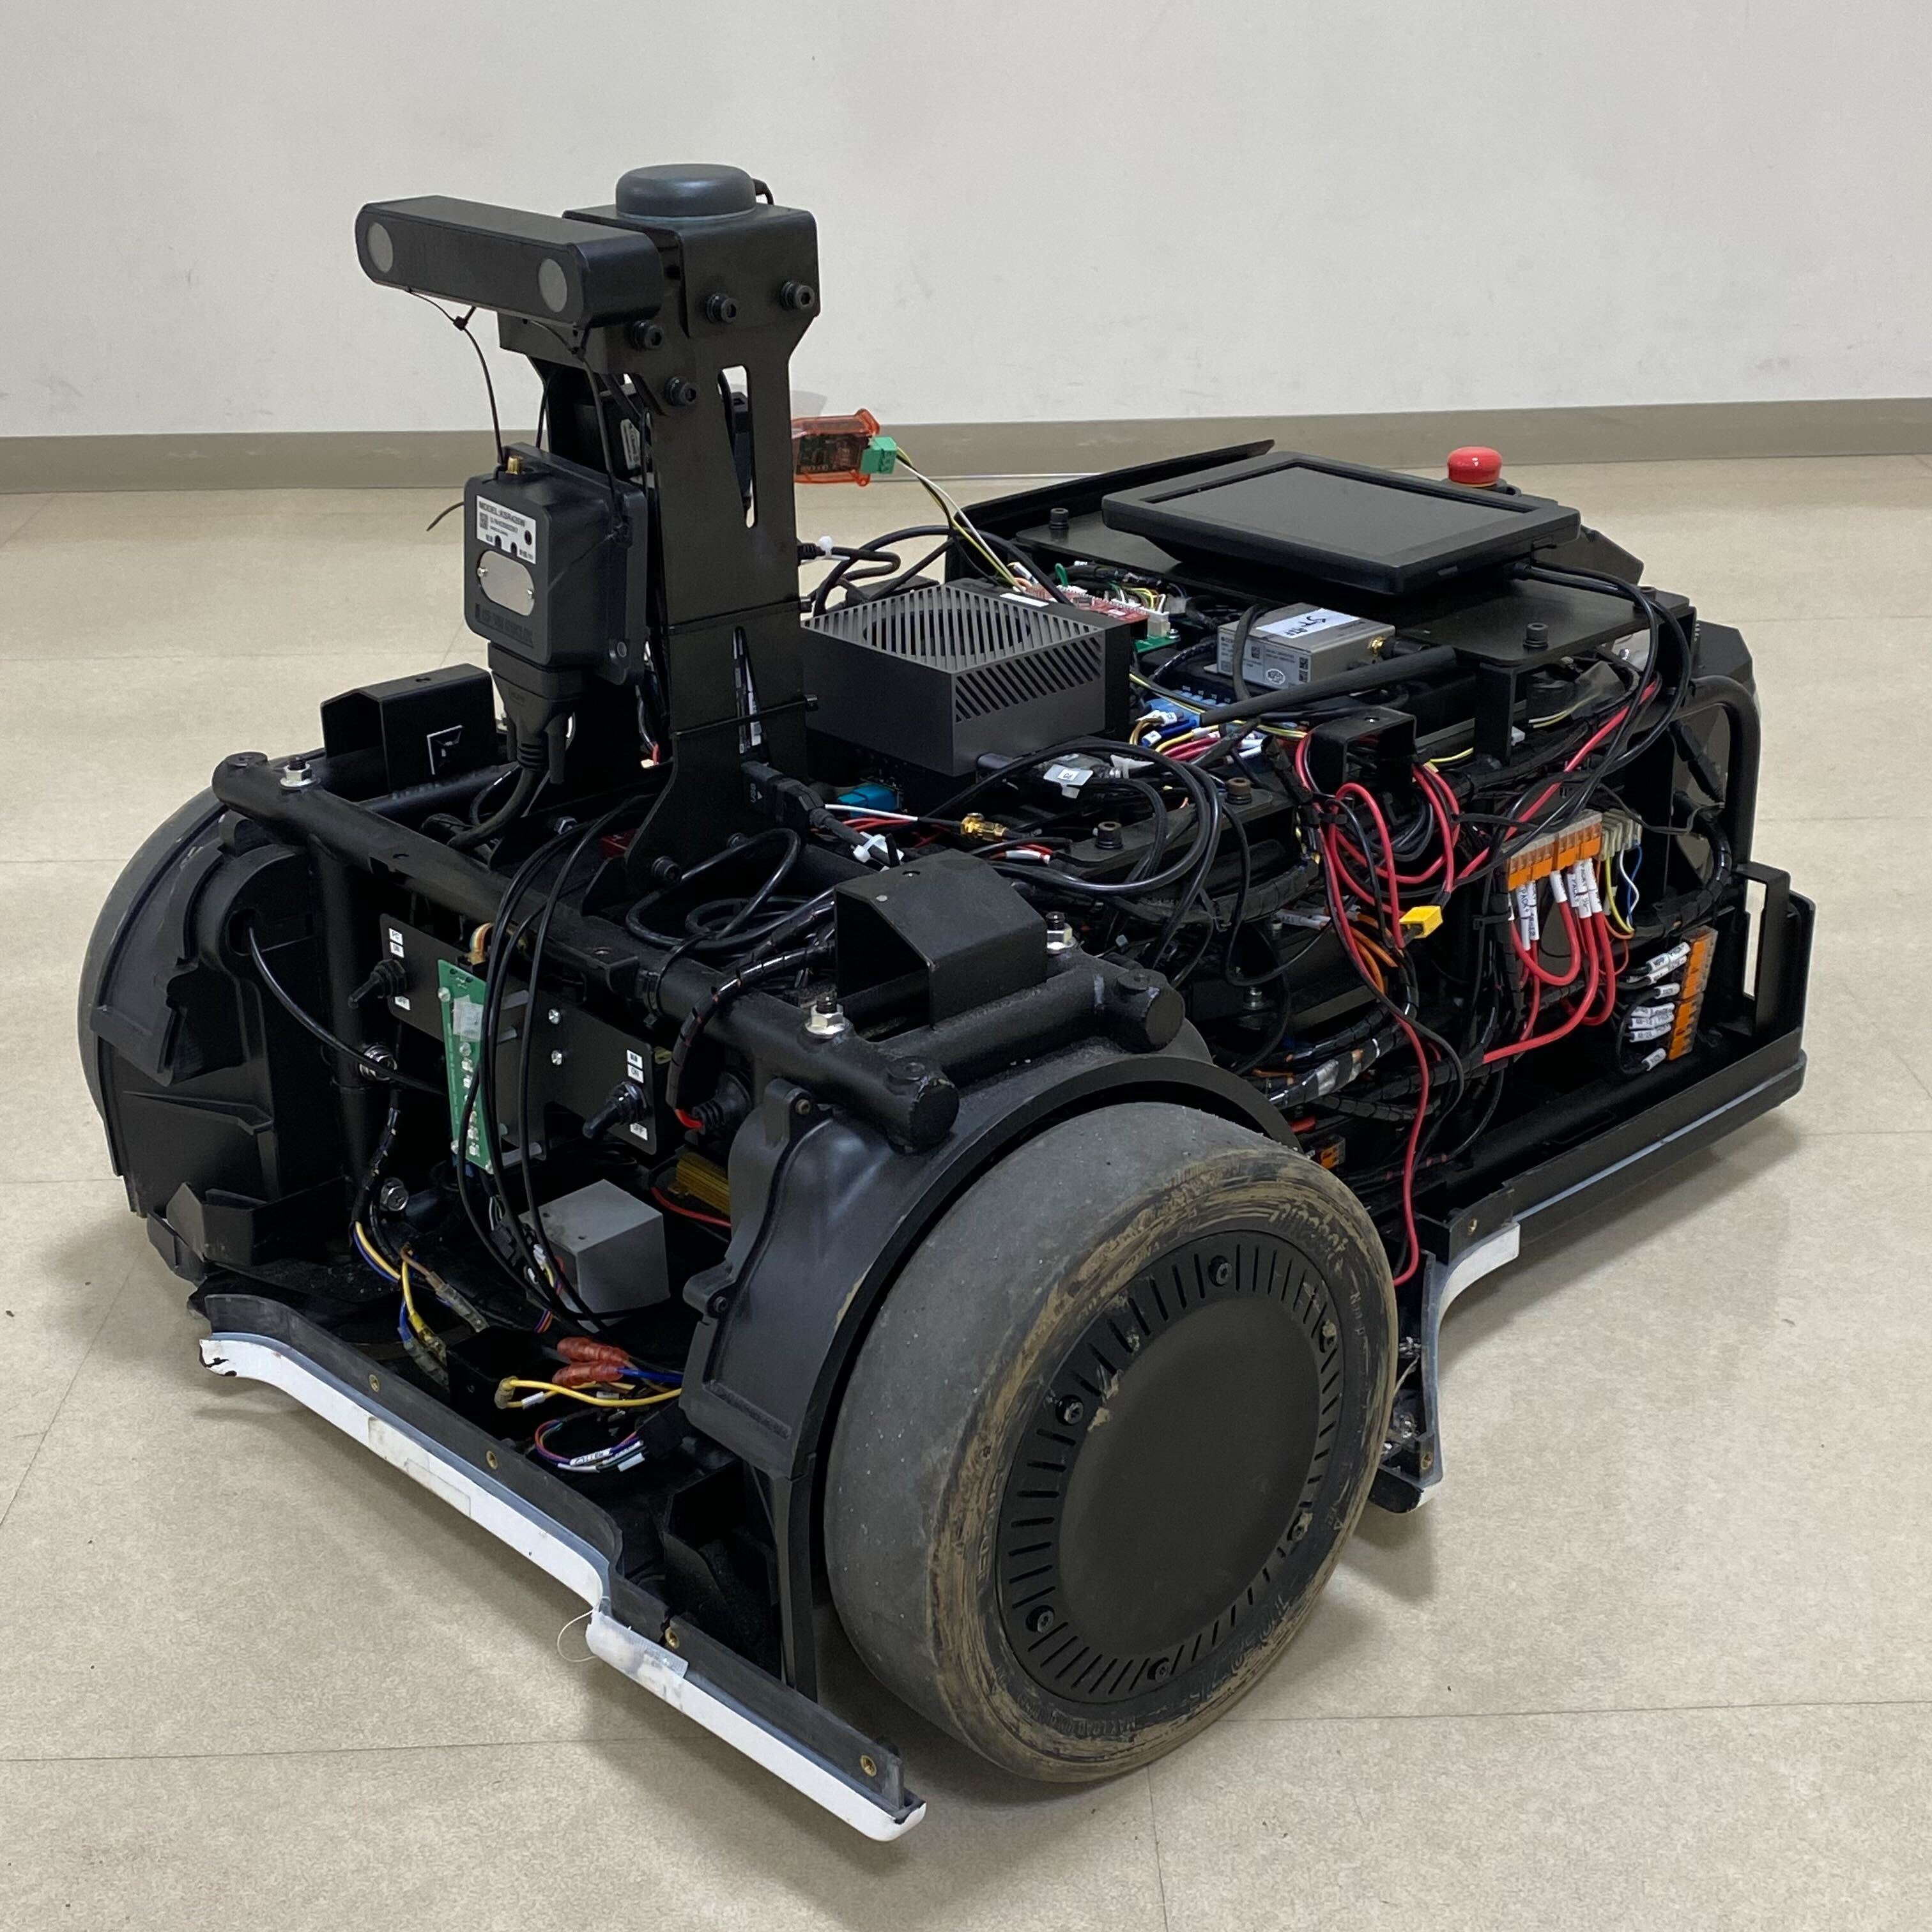
\includegraphics[height=50mm]{images/robotwithoutexterior.png}
         \subcaption{Mobility without exterior}
     \end{minipage}
     \caption{Robot appearance}
     \label{Fig:RobotGuidance_velocity}
\end{figure}

\subsection{センサ構成}
モビリティに搭載されているセンサ構成について述べる.
貸与されたモビリティにはステレオカメラ, GNSS+IMU, ホイールエンコーダなどのセンサが搭載されている.
開発するソフトウェアではGNSS+IMUセンサ(VectorNav VN-200)を使用する.

Fig.3.2にモビリティのセンサと位置を示す.

\begin{figure}[H]
     \centering
    \includegraphics[keepaspectratio, scale=0.7]
         {images/sensordescription.png}
    \caption{Mobility description}
    \label{fig:MPP}
\end{figure}

\subsubsection{VN-200}
VN-200\cite{vn-200}はGNSSとIMUを内包したセンサーであり, 3軸ジャイロ, 加速度計, 磁力系, GNSS受信機を用いて位置, 速度, 姿勢を推定することができる小型で高性能なGNSS支援慣性航法システムである.
IMUを内包しているため, 位置だけでなく方位も取得できるセンサとなっている.
VectorNavの方位は2種類の情報を手がかりに補正されるようになっており, 起動時は地磁気を手がかりに, 移動後はGNSSの履歴を手がかりに補正される.
ROS 2のラッパーとして, vectornavというパッケージが公開されている.\cite{vectornav}
Fig.3.3にVN-200の外観を示す.

\begin{figure}[H]
  \centering
 \includegraphics[keepaspectratio, scale=0.6]
      {images/vn-200.png}
 \caption{VectorNav VN-200 (source : [6])}
 \label{fig:vn-200 view}
\end{figure}

\subsection{従動輪}
貸与されたモビリティには従動輪の向きが望む方向に変化しない問題が発生していたため, 従動輪の向きをモータで駆動することで対処した.
これを実装したモビリティは結果的に, 高い操縦性により望む方向に移動できるようになった.
Fig.3.4に機構を示す.

% \phi= \arcsin\left(\frac{W\omega}{v}\right)

\begin{figure}[H]
  \centering
 \includegraphics[keepaspectratio, scale=0.5]
      {images/caster.png}
 \caption{Mechanism for driving the caster orientation}
 \label{fig:Mechanism for driving the caster orientation}
\end{figure}

\subsection{ブレーキ機構}
ブレーキ機構にはディスクブレーキと回生ブレーキが使用されている.
ディスクブレーキ機構はステッピングモータでディスクブレーキのワイヤを引っ張ることでブレーキがかかる機構となっている.

% \section{システム構成}
% ここで, 経路追従に用いることができるセンサはステレオカメラに加えてGNSSがある.
% 2つのセンサを比べたとき, 扱いの用意さという点ではGNSSに軍配があがる.
% ただし, マルチパスなどによる経緯度の誤差は数10mにおよぶことがあるため, 必ずしも経路追従に利用できるとは限らない.
% 幸いにして, AIFormulaの会場であるAIモビリティパークの周囲には高い建物が無く, マルチパスの影響が少ないと考えられた.
% そのため, GNSSに基づいた経路追従を行うシステムを開発した.
% Fig.4.4に経路追従で使用するシステム構成を示す.

% \begin{figure}[H]
%   \centering
%  \includegraphics[keepaspectratio, scale=0.2]
%       {images/system.png}
%  \caption{Path following system}
%  \label{fig:system}
% \end{figure}

% GNSSを用いて経路追従を行うためには, 位置に加えて方向のデータも必要となる.
% モビリティに搭載されているGNSS+IMU(VectorNav VN-200)は方位も計測できる仕様であるため, それを利用することが開発の多重化を防ぐ意味で望ましいと判断した.
% GNSS+IMU(VectorNav VN-200)はvectornav\cite{vectornav}というパッケージが公開されているため, そちらを使用してVectornavのセンサデータをROS 2 topicとして扱っている.
% 作成した経路追従のソフトウェアは, 事前にシュミレータ環境や手動走行をさせた時のGNSSから得た座標データをCSVファイルに経路情報としてまとめている.
% 用意した経路情報は測地座標系でまとめられていて, プロセスを起動したときにUTM座標系に変換されて目標経路の情報を含んだROS 2 topicとしてpublishされる.
% 経路追従を行うに際して, 自己位置はGNSSから取得した座標データをそのまま自己位置として扱っている.
% 取得した座標系はECEF座標系で取得されるため, 目標経路の座標系と合わせるためにUTM座標系に変換する.
% UTM座標系に合わされた目標経路の座標と自己位置の座標を利用してPurePursuitによる経路追従を行う.
% PurePursuitによって目標地点との角度差を取得し, その角度差に対してPID制御を行うことでモビリティの角速度を決定する.
% 並進速度は一定として, 求めた角速度に基づいてモビリティを制御する.

% \section{目標経路の作成}
% 経路追従をする際には追従するための目標経路が必要となる.
% 本研究では, 以下の図に示すように予め取得した経緯度のウェイポイントをつなぐライン状を移動する目標位置をPurePursuitで求め, 求めた目標地点に向かって進む制御を採用した.
% 経路情報はシミュレータ環境や事前に手動走行させたときのGNSSから得た情報を参照している.
% Fig.4.5に作成した目標経路の例を示す.

% \begin{figure}[H]
%   \centering
%  \includegraphics[keepaspectratio, scale=0.3]
%       {images/targetpath.png}
%  \caption{Predefined target trajectory}
%  \label{fig:target path}
% \end{figure}

\newpage